A figura reúne estas cinco ligações. Cada caixa de multiplicação
recebe dois fios. O nome escrito em cada fio refere a posição
efectiva que lhe cabe na porta. A soma da direita é uma relação
linear nos resultados. O provador pode, por isso, descrevê-la
sem acrescentar uma terceira porta de multiplicação.
\begin{center}
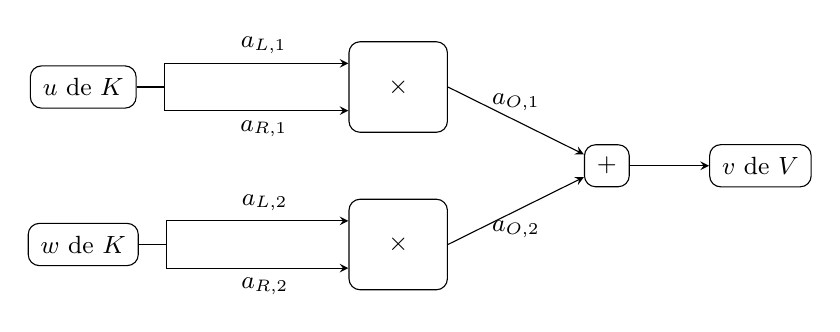
\begin{tikzpicture}[>=stealth,font=\small,
 block/.style={draw,rounded corners,align=center,inner sep=4.5pt}]
 \node[block] (u) at (-4.5,1) {\(u\) de \(K\)};
 \node[block] (w) at (-4.5,-1) {\(w\) de \(K\)};
 \node[block,minimum height=1.15cm,minimum width=1.25cm] (p) at (-.5,1) {\(\times\)};
 \node[block,minimum height=1.15cm,minimum width=1.25cm] (q) at (-.5,-1) {\(\times\)};
 \node[block] (sum) at (2.15,0) {\(+\)};
 \node[block] (v) at (4.1,0) {\(v\) de \(V\)};
 \draw[->] (u.east)--++(.35,0)|- ([yshift=3mm]p.west)
   node[pos=.77,above] {\(a_{L,1}\)};
 \draw[->] (u.east)--++(.35,0)|- ([yshift=-3mm]p.west)
   node[pos=.77,below] {\(a_{R,1}\)};
 \draw[->] (w.east)--++(.35,0)|- ([yshift=3mm]q.west)
   node[pos=.77,above] {\(a_{L,2}\)};
 \draw[->] (w.east)--++(.35,0)|- ([yshift=-3mm]q.west)
   node[pos=.77,below] {\(a_{R,2}\)};
 \draw[->] (p.east)--node[midway,above] {\(a_{O,1}\)} (sum);
 \draw[->] (q.east)--node[midway,below] {\(a_{O,2}\)} (sum);
 \draw[->] (sum)--(v);
\end{tikzpicture}
\end{center}

Retenhamos a disposição da figura e perguntemos o que terá de fixar
uma descrição pública deste circuito. O primeiro fio pode receber
qualquer elemento do corpo, mas a sua origem é a primeira coordenada
de \(K\). O segundo recebe a mesma coordenada e leva-a ao segundo operando da porta. O verificador
pode numerar os fios e indicar de antemão onde começa e onde acaba
cada um. Nesta descrição a posição de um valor é pública. O valor
que Alice escreverá nessa posição pertence à sua testemunha.

Tomemos por ordem os seis números das portas e os três números
comprometidos. Escrevamos o vector das suas posições como
\[
 \boldsymbol z_0=(a_{L,1},a_{L,2},a_{R,1},a_{R,2},
                      a_{O,1},a_{O,2},u,w,v)^\top .
\]
Esta letra com índice zero designa apenas as nove posições deste
quadro. As cinco linhas seguintes descrevem os fios. Uma entrada
\(1\) conserva o sinal da posição respectiva e uma entrada
\(-1\) subtrai-a. Os espaços em branco valem zero.
\[
\begin{array}{c|rr|rr|rr|rr|r}
 &a_{L,1}&a_{L,2}&a_{R,1}&a_{R,2}&a_{O,1}&a_{O,2}&u&w&v\\ \hline
 1&1&&&&&&-1&&\\
 2&&&1&&&&-1&&\\
 3&&1&&&&&&-1&\\
 4&&&&1&&&&-1&\\
 5&&&&&1&1&&&-1
\end{array}
\]
Designemos a matriz por \(M\). Para a testemunha dos quadrados,
o vector que ela multiplica é \((3,4,3,4,9,16,3,4,25)^\top\).
Ler o quadro na horizontal dá \(3-3,3-3,4-4,4-4,9+16-25\).
É essa a igualdade \(M\boldsymbol z_0=\boldsymbol0\). Já o
produto de cada porta lê-se na vertical entre posições
correspondentes dos três primeiros pares de colunas. Combinar as
descrições obriga o três a chegar a ambos os operandos da primeira
porta, o quatro a chegar a ambos os operandos da segunda e a soma
dos quadrados a terminar no compromisso escalar.

Há ainda outra leitura, particularmente económica para quem
verifica. Demos pesos \(q_1,\ldots,q_5\) às linhas e somemo-las.
Para saber que parte da combinação vem de \(u\), basta percorrer a
coluna de \(u\). Duas linhas lhe atribuíram \(-1\), pelo que lhe cabe o coeficiente \(-q_1-q_2\). A coordenada \(w\) recebe
\(-q_3-q_4\). Ao valor \(v\) chega só \(-q_5\), e ambos os
resultados das portas recebem \(+q_5\). Podemos ler de uma vez
a combinação inteira
\[
 \begin{aligned}
 &q_1a_{L,1}+q_3a_{L,2}
     +q_2a_{R,1}+q_4a_{R,2}
     +q_5(a_{O,1}+a_{O,2})\\
 &\hspace{18mm}-(q_1+q_2)u-(q_3+q_4)w-q_5v .
 \end{aligned}
\]
Substituir a testemunha honesta anula a expressão quaisquer que
sejam os pesos. O ponto de vista do verificador é o inverso.
Sendo-lhe ocultas as entradas do vector, ele prepara a combinação
por meio dos coeficientes das colunas. O que poderá calcular com
as bases públicas e os compromissos será justamente uma igualdade
que contenha essa combinação. A transposta da matriz irá aparecer
porque reúne, numa só operação, os pesos de todas as linhas por onde
passa cada coordenada.

Vejamos essa troca com números. Ponhamos
\((q_1,q_2,q_3,q_4,q_5)=(2,4,8,16,32)\). A combinação das linhas
atribui \(-6\) à primeira coordenada de \(K\) e \(-24\) à segunda.
Percorrendo as ligações com as aberturas \(u=3,w=4\), chegam
\(2\cdot3+8\cdot4=38\) pelo lado esquerdo das portas e
\(4\cdot3+16\cdot4=76\) pelo lado direito. A parcela de \(K\)
vale \(-6\cdot3-24\cdot4=-114\), que cancela exactamente
\(38+76\). Pelos resultados chegam \(32(9+16)=800\), e no valor
de \(V\) espera-os \(-32\cdot25=-800\). Pode fazer-se esta conta
nos inteiros e tomar o resultado no corpo de escalares. Para qualquer
número de portas, a cada ocorrência de uma
variável corresponde uma entrada na matriz, e os contributos de
todas as suas ocorrências juntam-se na coluna que lhe cabe.

Os compromissos exteriores dão a estas ligações uma consequência
observável. \(3^2+4^2\) e \(4^2+3^2\) dão ambos \(25\).
A declaração que conhece somente o resultado admite ambas as ordens
dos operandos. No compromisso \(K\), contudo, a primeira coordenada
multiplica \(g_1\) e a segunda multiplica \(g_2\). Mantida a
máscara, passar de \((3,4)\) para \((4,3)\) desloca o ponto por
\(g_1-g_2\). O circuito tem, por isso, uma razão para dar nome
próprio às duas posições, mesmo ao efectuar uma soma simétrica.
Está a demonstrar que a relação vale para os valores que entraram
naqueles lugares dos compromissos publicados.
